%
% Morse-Theorie
%
\section{Morse-Theorie
\label{buch:topologie:section:morse}}
\kopfrechts{Morse-Theorie}
Die Morse-Theorie stellt einen Zusammenang zwischen der Topologie einer 
Mannigfaltigkeit und den kritischen Punkten einer Funktion auf der
Mannigfaltigkeit.
Die grössräumigen Eigenschaften einer Mannigfaltigkeit sind also
in den Eigenschaften von Funktionen in einigen wenigen, isolierten
Punkten einer Funktion codiert.

%
% Zerlegung einer zweidimensionalen Mannigfaltigkeit
%
\subsection{Zerlegung einer zweidimensionalen Mannigfaltigkeit}
%
% fig-karte.tex
%
% (c) 2025 Prof Dr Andreas Müller
%
\begin{figure}
\centering
\includegraphics[width=\textwidth]{chapters/120-topologie/images/karte.png}
\caption{Die Hähenlinien sind die Niveaulinien der auf der Erdoberfläche
definierten Funktion, die die Höhe eines Punktes angibt.
Die Niveaulinien zerlegen die Oberfläche der Erde in Streifen oder Ringe.
Die Idee der Morse-Theorie ist, dass sich die Topologie der Erdoberfläche
aus diesen Elementen rekonstruieren lässt.
\label{buch:topologie:morse:fig:karte}}
\end{figure}
%
%
% fig-relief.tex
%
% (c) 2025 Prof Dr Andreas Müller
%
\begin{figure}
\centering
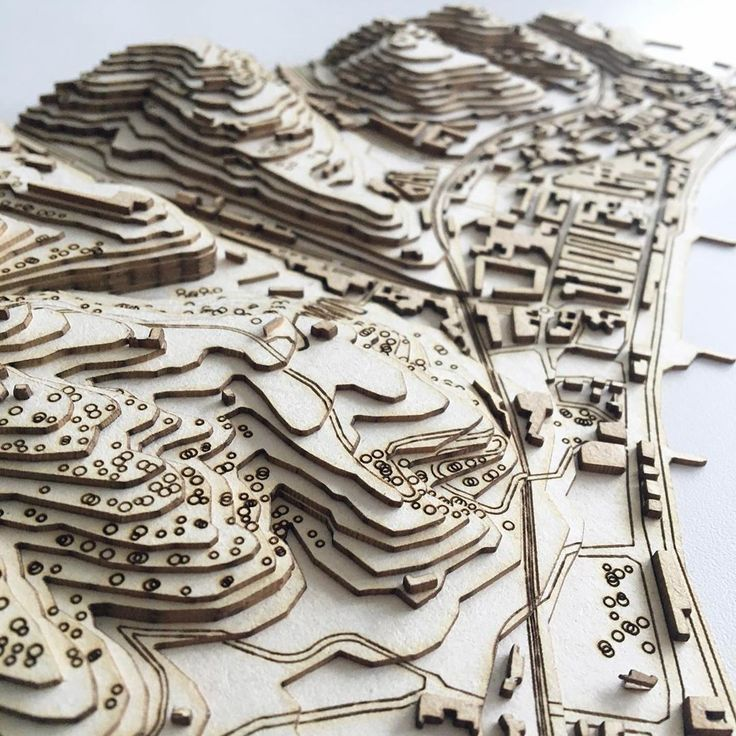
\includegraphics[width=0.7\textwidth]{chapters/120-topologie/images/relief.jpg}
\caption{Rekonstruktion einer Approximation der Topographie aus den
\index{Topographie}%
Höhenlinien mit Hilfe von Platten, die entlang der Höhenlinien ausgeschnitten
worden sind.
\label{buch:topologie:morse:fig:relief}}
\end{figure}
%
Aus einer glatten Funktion $f\colon M\to\mathbb{R}$ lässt
sich eine natürliche Zerlegung einer Mannigfaltigkeit konstruieren.
In Abbildung~\ref{buch:topologie:morse:fig:karte} zeigt eine 
topographische Karte.
Die Höhenlinien sind die Niveaulinien der Funktion, die einem
Punkt seine Höhe über dem Meeresspiegel zuordnet.
Die Höhenlinien zerlegen die Karte in Streifen, Ringe und andere
zweidimensionale Gebiete.
Der geübte Kartenleser ist in der Lage, aus den Höhenlinien eine
Vorstellung der Topographie zu rekonstruieren.
Man kann aber auch aus den Höhenlinien ein massstäbliches Modell
des Geländes rekonstruieren.
Für jedes Niveau schneidet man das von der Höhenlinie berandete Gebiet
aus einer Holzplatte aus und schichtet die erhaltenen Platten
wie in Abbildung~\ref{buch:topologie:morse:fig:relief} gezeigt
auf.
Es entsteht eine Approximation des Geländes.

Wir betrachten jetzt eine einzelne Höhenlinie.
Die Höhenlinie zur Höhe $c$ ist die Menge der Punkte
\[
H_c
=
\{ p\in M\mid f(p) = c \}.
\]
Wenn wir $c$ um einen kleinen Betrag $\Delta c$ verschiebt sich
die Höhenlinie in eine Richtung senkrecht auf die Höhenlinie.
Ein positives $\Delta c$ bedeutet, dass wir eine Höhenlinie weiter
oben am Berg suchen.
Ist $\Delta c$ klein genug, ist die neue Höhenlinie $H_{c+\Delta c}$
meistens eine Kurve, die in unmittelbarer Nähe der Kurve $H_c$.
die Veränderung von $c$ hat also keine wesentlichen Auswirkungen
auf die Gestalt der Höhenlinie, wenigstens wenn die Höhenlinie
immer an einem Hang entlang verläuft.

Die Voraussetzung, dass die Höhenlinie dem Hang entlang verlaufen
muss, damit einen kleine Höhenänderung keine Auswirkung auf die
Gestalt der Kurve hat, ist zum Beispiel bei einem Gipfel verletzt.
Sei $p$ ein lokales Maximum der Funktion $f$ und U eine so kleine
Umgebung von $p$, dass die Höhenlinie $H_c = \{p\}$ nur den Punkt $p$
enthält.
Vergrössert man $c$ um $\Delta c>0$, verschwindet der Punkt $p$,
die Höhenlinie $H_{c+\Delta c}=\emptyset$ ist leer.
Bei einer Verkleinerung wird wird die Höhenline $H_{c+\Delta c}$ zu
einer geschlossenen Kurve, die den Punkt $p$ umschliesst
(Abbildung~\ref{buch:topologie:morse:fig:karte}, Umgebung des Punktes 1384),
wenigstens wenn die zweiten Ableitungen von $f$ an der Stelle $p$
nicht verschwinden.

Ein ganz anderes Bild bietet sich bei einem Pass der Höhe $c$.
Auch ein Sattelpunkt der Fläche ist eine Stelle, an der
alle partiellen ersten Ableitungen verschwinden.
Die Menge $H_c$ besteht aber nicht aus einem Punkt, vielmehr
kommen im Punkt $p$ vier Höhenlinien zusammen.
Für grössere und kleiner Werte verschwindet der Schnittpunkt,
es bleiben zwei nicht verbundene Höhenlinie wie in
bei links unterhalb der Büelhöchi in
Abbildung~\ref{buch:topologie:morse:fig:karte}.

Diese Diskussion zeigt, dass wesentliche Eigenschaften der Topographie
aus Punkten abzulesen sind, an denen die ersten Ableitungen verschwinden,
die zweiten Ableitungen aber nicht (was das genau heisst, muss noch
definiert werden).

%
% Index einer Nullstelle
%
\subsection{Kritische Punkte und ihr Index}
In diesem Abschnitt ist $M$ eine $n$-dimensionale Mannigfaltigkeit.
Wir betrachten die Menge $C^\infty(M)$ der beliebig oft stetig
differenzierbare Funktionen auf $M$.

%
% Kritische Punkte
%
\subsubsection{Kritische Punkte}
%
% fig-morse.tex
%
% (c) 2025 Prof Dr Andreas Müller
%
\begin{figure}
\centering
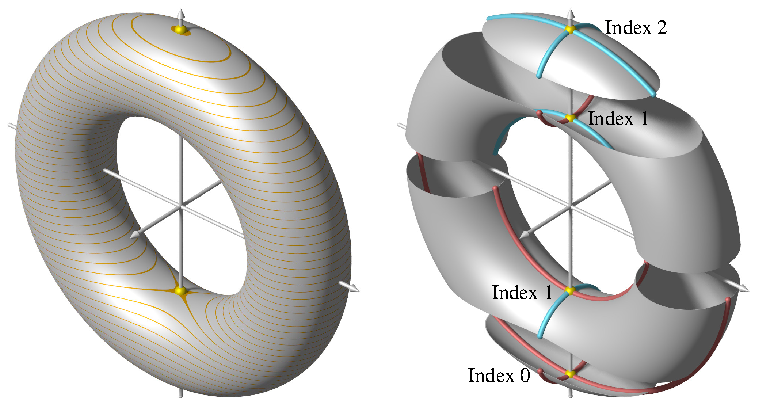
\includegraphics{chapters/120-topologie/images/morse.pdf}
\caption{Links: Torus mit Höhenlinien der Funktion $f(p) = z(p)$ für Punkte
$p$ auf dem Torus.
\index{Torus}%
Kritische Punkte von $f$ sind gelb eingezeichnet.
\index{kritischer Punkt}%
Rechts: Der Torus lässt sich in Teile zerlegen, die jeweils genau
einen kritischen Punkte enthalten. Aus den Indizes der kritischen Punkte
\index{Index}%
lassen sich topologische Eigenschaften der Mannigfaltigkeit rekonstruieren.
\label{buch:topologie:fig:morse}}
\end{figure}
%
Die äussere Ableitung einer Funktion $f\colon M\to\mathbb{R}$ 
wird ein einer Karte $\varphi_\alpha\colon U_\alpha\to\mathbb{R}^n$
zu einer Funktion der $n$ Koordinaten, die wir $f(x^1,\dots,x^n)$
schreiben.
Bei einem Maximum oder Minimum der Funktion verschwinden alle ersten
Ableitungen, in dieser Karte wird die äussere Ableitung
\[
df
=
\frac{\partial f}{\partial x^1}\,dx^1
+
\dots
+
\frac{\partial f}{\partial x^n}\,dx^n
=
0.
\]
Wechselt man das Koordinatensystem, ändert dies an der Tatsache, dass
$df=0$ ist, nichts.

\begin{definition}[kritischer Punkt]
\index{kritischer Punkt}%
\index{Punkt!kritisch}%
\index{kritischer Wert}%
\index{Wert!kritisch}%
Ein \emph{kritischer Punkt} einer glatten Funktion $f$ auf einer
differenzierbaren Mannigfaltigkeit ist ein Punkt $p\in M$, bei dem
$df(p)=0$ ist.
Der Wert $c=f(p)$ in einem kritischen Punkt $p$ heisst
\emph{kritischer Wert} der Funktion f.
\end{definition}

%
% Die hessesche Matrix
%
\subsubsection{Die hessesche Matrix}
Sei $p$ ein kritischer Punkt der Funktion $f$ auf der Mannigfaltigkeit $M$
mit dem kritischen Wert $c=f(p)$.
In einem Koordinatensystem in der Umgebung des Punktes $p$ kann die Funktion
durch die Taylor-Reihe 
\begin{align}
f(x^1,\dots,x^n)
&=
f(p)
+
\sum_{k=1}^n \frac{\partial f}{\partial x^k}(p) (x^k-x^k(p))
\\
&\qquad\mathstrut
+
\sum_{k,l=1}^n
\frac{\partial^2 f}{\partial x^k\,\partial x^l}(p)
(x^k-x^k(p))(x^l-x^l(p))
+
o(|x-p|^2)
\notag
\\
&=
c
+
\sum_{k,l=1}^n
\frac{\partial^2 f}{\partial x^k\,\partial x^l}(p)
(x^k-x^k(p))(x^l-x^l(p))
+
o(|x-p|^2)
\label{buch:topologie:morse:eqn:quadratisch}
\end{align}
approximiert werden.
Die Matrix der zweiten Ableitungen heisst auch die hessesche Matrix $H$
an der Stelle $p$ mit den Einträgen
\[
h_{ik}
=
\frac{\partial^2 f}{\partial x^i\,\partial x^k}(p).
\]

In einer Dimension besteht die hessesche Matrix nur aus der zweiten
Ableitung $f''(p)$ der Funktion.
Wenn Sie nicht verschwindet lässt sich daraus ableiten, ob der
kritische Punkt ein lokales Maximum oder Minimum ist.
In höheren Dimensionen ist die Situation etwas komplizierter

%
% Nichtentartete quadratische Formen
%
\subsubsection{Nichtentartete quadratische Formen}
Wir möchten sicherstellen, dass wir zuverlässige Aussagen über die
Form der \emph{Niveaumengen} $H_c=\{p\in M\mid f(p)=c\}$ in der
Umgebung eines kritischen Punktes machen können.
Dazu muss der quadratische Term in
\eqref{buch:topologie:morse:eqn:quadratisch}
immer gegenüber den Termen höherer Ordnung dominieren.
Dies ist nur möglich, wenn der quadratische Ausdruck
\[
H(v)
=
\sum_{k,l=1}^n
\frac{\partial^2 f}{\partial x^k\,\partial x^l}
v^k v^l
\]
nicht entartet im Sinne der folgenden Definition ist.

\begin{definition}[quadratische Form]
Ist $H$ eine symmetrische Matrix, dann ist schreiben wir
\[
H(v)
=
v^tHv
=
\sum_{i,k=1}^n = h_{ik} v^iv^k
\]
und sagen, dass $H(v)$ eine \emph{quadratische Form} ist.
\end{definition}

Die \emph{Polarisationsformel} \cite[p.~347]{buch:linalg} ermöglicht,
aus der quadratischen Form
\index{Polarisierungsformel}
$H(v)$ die Bilinearform
\[
\langle u,v\rangle_H
=
u^tHv
\]
zu rekonstruieren.
Die Formel lautet
\[
\langle u,v\rangle_H
=
\frac14\bigl(H(u+v) - H(u-v)\bigr).
\]
Damit können jetzt auch die Matrixelemente
$h_{ik} = \langle\vec{e}_i,\vec{e}_k\rangle_H$ von $H$
wiedergewinnen.
Man verliert also nichts, wenn man nur die quadratische Form kennt,
wie sie in der Taylor-Reihe auftritt.

\begin{definition}[entartete quadratische Form]
\label{buch:topologie:morse:def:entartet}
Eine quadratische Form mit Matrix $H$ heisst \emph{entartet}, wenn
die Matrix $H$ singulär ist.
\end{definition}

Die Bedingung der Definition~\ref{buch:topologie:morse:def:entartet}
bedeutet, dass es einen Vektor $v$ mit $Hv=0$ gibt.
Für einen solchen Vektor gilt $\langle u,v\rangle_H=0$
für alle Vektoren $u$.
Die Bedingung verhindert nicht, dass es Vektoren gibt, für die
$H(u)=0$.
Die quadratische Form mit der Matrix
\[
H=
\begin{pmatrix}
1&0\\0&-1
\end{pmatrix}
\]
ist sicher nicht entartet, aber wegen
\[
v^tHv
=
(v^1)^2-(v^2)^2
\]
gilt
\[
v=\begin{pmatrix}1\\1\end{pmatrix}
\qquad\Rightarrow\qquad
H(v) = 0.
\]
Es gibt also eine Richtung, für die die quadratische Form verschwindet.
Für die Standardbasisvektoren gilt allerdings
$ H(e_1)=1$ und $H(e_2)=-1$.
Die Funktion $z=H(v^1,v^2)$ kann als Sattelfläche dargestellt werden.
Auf einer Sattelfläche gibt es Richtungen, in denen sich $H$ nicht
verändert und Richtungen, für die $H$ zu- bzw.~abnimmt.

Die Bedingung, dass die hessesche Matrix $H$ nicht entartet sein darf,
entspricht der Bedingung für Funktionen einer Variablen, dass die zweite
Ableitung nicht verschwinden darf.
Sie stellt sicher, dass der quadratische Term in der Nähe des kritischen
Punktes in alle Richtungen das Vorhalten der Funktion dominiert.

%
% Der Index eines kritischen Punktes
%
\subsubsection{Der Index eines kritischen Punktes}
Die hessesche Matrix $H$ mit den Einträgen
\[
h_{kl} = \frac{\partial^2 f}{\partial x^k\,\partial x^l}
\]
ist in einem nicht entarteten kritischen Punkt eine symmetrische
Matrix.
Da symmetrische Matrizen durch orthogonale Transformationen
diagonalisierbar sind, können wir das Koorinatensystem mit
einer orthogonalen Matrix so drehen, dass $H$ die Form
\[
H(v)
=
\sum_{i=1}^n \lambda_i (v^i)^2
\]
bekommt.
Die $\lambda_i$ sind die Eigenwerte der Matrix $H$, keiner
der Eigenwerte verschwindet.
Durch Streckung der Koordinatenachse $x^1$ mit dem Faktor
$\!\sqrt{|\lambda_i|}$  mittels
$y^i = \!\sqrt{|\lambda_i|}x^i$ kann die Entwicklung
\eqref{buch:topologie:morse:eqn:quadratisch}
in die Form
\begin{align*}
f(y^1,\dots,y^n)
&=
c
+
\operatorname{sgn}(\lambda_1)\,(y^1)^2
+
\dots
+
\operatorname{sgn}(\lambda_n)\,(y^n)^2.
\end{align*}
Es kommt also nur auf die Vorzeichen der Eigenwerte an.
Bei einem Koordinatenwechsel ändert sich die Matrix $H$ der zweiten
Ableitungen, aber die Anzahl der positiven und negativen Eigenwerte
bleibt erhalten.

\begin{definition}[Index]
\index{Index einer quadratischen Form}%
Der \emph{Index} einer nicht entarteten quadratischen Form $H$ ist die
Anzahl $k$ der negativen Eigenwerte.
Der Index wird mit $\operatorname{Ind}H$ bezeichnet.
\end{definition}

Der Index ist eine Grösse, die auf kleine Störungen der Funktion
unempfindlich ist, solange der Punkt ein kritischer Punkt bleibt.

%
% Morse-Funktionen
%
\subsubsection{Morse-Funktionen}
Wir betrachten die Funktion
\[
f_t(x)
=
x^3-tx
=
(x-\!\sqrt{t})x(x+\!\sqrt{t})
\]
mit dem Parameter $t$, wobei die Faktorisierung nur für $t\ge 0$ möglich
ist.
Die Ableitungen sind
\begin{align*}
f'_t(x)
&=
3x^2-t
=
(\!\sqrt{3}x-\!\sqrt{t})
(\!\sqrt{3}x+\!\sqrt{t})
\\
f''_t(x)
&=
6x.
\end{align*}
Für $t> 0$ hat die Funktion zwei kritische Punkte bei $\pm\!\sqrt{t/3}$,
die nicht entartet sind, weil die zweite Ableitung $\ne 0$ ist.
Die beiden kritischen Punkte haben verschiedenen
Index $0$ für $t=\!\sqrt{t/3}$
und $1$ für $t=-\!\sqrt{t/3}$.
Für $t<0$ gibt es keine kritischen Punkte.
Für $t=0$ gibt es den kritischen Punkt $x=0$, der aber entartet ist.
Die Differenz der Anzahl positiver und negativer zweiter Ableitungen
bei den kritischen Punkten bleibt bei der Deformation der Funktion 
mithilfe des Paramters $t$ gleich.
Dies suggeriert, dass die Betrachtung der kritischen Punkte etwas
über die topologischen Eigenschaften aussagt.
Dies funktioniert aber nicht für den Fall $t=0$, weil der kritische
Punkt dort entartet ist.
Für die topologische Untersuchung sind daher nur Funktionen geeignet,
die keine entarteten kritischen Punkte haben.

\begin{definition}[Morse-Funktion]
\index{Morse-Funktion}%
Eine {\em Morse-Funktion} auf einer differenzierbaren Mannigfaltigkeit
$M$ ist eine stetig differenzierbare Funktion $f\colon M\to\mathbb{R}$,
deren kritische Punkte alle nicht entartet sind.
Der Index $\operatorname{Ind}_pf$ des kritischen Punktes ist der Index
der hesseschen Matrix im Punkt $f$:
\[
\operatorname{Ind}_pf
=
\operatorname{Ind}\biggl(
\frac{\partial^2 f}{\partial x^i\,\partial x^k}(p)
\biggr).
\]
\end{definition}

Nach obiger Diskussion ist das Einführungsbeispiel $f_t(x)$ also für
$t\ne0$ eine Morse-Funktion auf $\mathbb{R}$.

Für Flächen $M$, die durch Einbettung in den dreidimensionalen Raum
$\mathbb{R}^3$ gegeben sind, sind die Koordinatenfunktion
$x(P)$, $y(P)$ und $z(P)$ natürlich Kandidaten für Morse-Funktionen.
Die Einbettung der Kugel
\[
S^2
=
\{ (x,y,z)\mid x^2+y^2+z^2=1 \}
\subset
\mathbb{R}^3
\]
liefert so drei Morse-Funktionen auf der Kugeloberfläche, die jeweils
genau zwei kritische Punkte mit Indizes 2 für das Maximum und
0 für das Minimum haben.
Man kann sich vorstellen, dass durch Deformation der Kugeln weitere
kritische Punkt der Koordinatenfunktionen entstehen können.
Ein zweites lokales Maximum wird aber immer mit einem Sattelpunkt
verbunden sein, der Index $1$ hat.

%\begin{definition}[Signatur eines kritischen Punktes]
%Sei $p$ ein kritischer Punkt der Morse-Funktion $f$.
%Die Signatur von $p$ ist
%\[
%\operatorname{sgn}_pf
%=
%n-2\operatorname{Ind}_pf
%\]
%Die Differenz der Anzahl der positiven bzw.~negativen Eigenwerte
%der hesseschen Matrix.
%\end{definition}
%
%Da die hessesche Matrix nicht entartet ist, ist die Anzahl der
%postiven Eigenwerte $n-\operatorname{Ind}_pf$ und damit die
%Differenz
%$n-\operatorname{Ind}_pf-\operatorname{Ind}_pf=n-2\operatorname{Ind}_pf$.
%Die Signatur ist positiv, wenn die hessische Matrix mehr positive als
%negative Eigenwerte hat.
%Die extremen Werte $\pm n$ werden erreicht, wenn alle Eigenwerte das
%gleiche Vorzeichen haben.
%
%Für das eindimensionale Einführungsbeispiel $f_t$ folgt, dass der kritische
%Punkt $\pm\!\sqrt{t/3}$ die Signatur $\mp 1$ hat.
%Die Summe der Signaturen ist eine Invariante unter der Deformation.
%
%Auf einer Fläche entspricht der Signatur $1$ ein lokales Minimum,

%
% Rekonstruktion
%
\subsection{Rekonstruktion}
Aus den Eigenschaften einer Morse-Funktion können viele topologische
Eigenschaften einer differenzierbaren Mannigfaltigkeit rekonstruiert
werden.
Die früher in Abschnitt~\ref{buch:topologie:section:homologie}
mit Hilfe der Homologiegruppen definierte Euler-Charakteristik
lässt sich zum Beispiel bereits mit aus einer Morse-Funktion
ableiten.

%
% Kugeln
%
\subsubsection{Kugeln}
Der folgende Satz zeigt, dass die Eigenschaften einer Morse-Funktion
tatsächlich bereits die topologischen Eigenschaften einer Mannigfaltigkeit
festlegen können.

\begin{satz}
\label{buch:topologie:morse:satz:kugeln}
Sei $M$ eine kompakte, $n$-dimensionale differenzierbare Mannigfaltigkeit
und $f$ eine Morse-Funktion mit genau zwei kritischen Punkten, dann ist
$M$ eine $n$-dimensionale Kugel.
\end{satz}

\begin{proof}
Man muss aus der Funktion $f$ eine bijektive differenzierbare Abbildung
von $M$ auf eine $n$-dimensionale Kugel konstruieren, deren Ableitung
in jedem Punkt regulär ist.

Da die Mannigfaltigkeit $M$ kompakt ist, nimmt $f$ auf $M$ mindestens
ein Maximum und ein Minimum an.
Diese sind automatisch kritische Punkte.
Weil $f$ eine Morse-Funktion ist, sind sie auch nicht entartet.
Wir bezeichnen den Punkt, in dem $f$ das Maximum annimmt, mit $N$,
und den Punkt, in dem $f$ das Minimum annimt mit $S$.
Durch Skalarierung der Funktion $f$ kann man ohne Beschränkung der
Allgemeinheit annehmen, dass $f(N)=1$ und $f(S) = -1$ ist.

Die Funktion $f$ kann als die $n+1$-Koordinate einer Abbildung von $M$ 
auf eine Kugel betrachtet werden.
Für die anderen Koordinatenfunktionen benutzen wir, dass wir annehmen
dürfen, dass es auf $M$ eine riemannsche Metrik gibt.
Mit ihre konstruieren wir das Vektorfeld $X$ des Gradienten der 1-Form $df$.

Sei jetzt $\gamma(t)$ eine Bahnkurve des Vektorfeldes durch einen Punkt
$p\in M$ mit der Eigenschaft $f(p)=0$.
Nach Definition des Vektorfeldes ist für jeden Wert $t$ im Definitionsbereich
von $\gamma$
\[
\frac{d}{dt}f\circ\gamma(t)
=
D_{\dot{\gamma}(t)} f
=
\langle df, \dot{\gamma}(t) \rangle.
\]
Durch Integration findet man, dass
\[
f(\gamma(t))
=
\int \langle df,\dot{\gamma}(t)\rangle \,dt
\]
ist.



Der Tangentialraum von $M$ im Punkt $N$ ist der
$n$-dimensionale Vektorraum $T_NM\equiv \mathbb{R}^n$.
Zu einem Einheitsvektor $\vec{v}$ 

\end{proof}

In diesem Zusammenhang ist auch der Satz von Poincaré-Bendixson,
der in Kapitel~\ref{chapter:poinbendix} vorgestellt wird, zu beachten.
Er besagt, dass ein Vektorfeld auf einer Kugeloberfläche $S^2$ nur
ganz bestimmte Lösungskurven haben kann.
Der Gradient einer Morse-Funktion wie in
Satz~\ref{buch:topologie:morse:satz:kugeln}
ist ein Vektorfeld mit nur zwei kritischen Punkten.
Für diesen Fall sagt der Satz von Poincaré-Bendixson, dass die
Lösungskurven Bahnen sind, die also $\omega$-Limesmengen die 
Maximumstelle haben, und als $\alpha$-Limesmenge die Minimumstelle.

%
% Homotopietyp und Morse-Funktion
%
\subsubsection{Homotopietyp und Morse-Funktionen}
Eine Morse-Funktion codiert in ihren kritischen Punkten Information
über die Struktur der Mannigfaltigkeit.
Auf einer kompakten Mannigfaltigkeit findet man immer einen kritischen
Punkt mit Index $0$ für die Minimumstelle und einen mit Indes $n$ für
das Maximum.
Weitere kritische Punkte treten auf für Sattelpunkte.

Abbildung~\ref{buch:topologie:fig:morse} zeigt einen zweidimensionalen
Torus.
Im ``Loch'' des Torus hat die $z$-Koordintenfunktion zwei kritische Punkte
mit Index $1$.
Die Abbildung zeigt auch, wie der Torus schrittweise aufgebaut werden
kann.
Man beginnt ganz unten mit einer Kreisscheibe.
Der nächsthöhere kritische Punkt zeigt an, dass zwischen zwei Punkten
des Randes eine Brücke gebaut werden muss.
Es entsteht jetzt eine Fläche mit zwei kreisförmigen Rändern.
Der nächste kritische Punkt zeigt an, dass die beiden Ränder mit
einer weiteren Brücke verbunden werden müssen.
Damit verschmelzen die beiden Randkreise wieder zu einem.
Schliesslich kann der Randkreis mit einer ``Kappe'' aus einer
zweidimensionalen Kreissscheibe geschlossen und damit eine
Mannigfaltigkeit konstruiert werden, die bis auf Deformation mit dem
Torus übereinstimmt.

Man nennt einen topologischen Raum, der schrittweise aus einem Punkt
durch Anfügen von $k$-dimensionaler Kreisscheiben aufgebaut werden kann,
einen CW-Komplex.
Die kritischen Punkte einer Morse-Funktion bestimmen einen solchen
Komplex bis auf Deformation.

%
% Euler-Charakteristik
%
\subsubsection{Euler-Charakteristik}
Die Diskussion kritischen Punkte auf dem Torus von
Abbildung~\ref{buch:topologie:fig:morse} hat gezeigt,
dass zum Index $0$ genau ein kritischer Punkt vorhanden ist,
zum Index $1$ deren zwei und zum Index 2 wieder einen.
Die Anzahl $n_k$ der kritischen Punkte mit Index $k$ stimmt in diesem Fall
also genau mit den Betti-Zahlen $\beta_k$ in Dimension $k$ überein.

Die Diskussion der kritischen Punkte auf der Kugeloberfläche
hat gezeigt, dass zusätzliche Maxima mit Sattelpunkten erkauft werden
können.
In diesem Fall stimmt die Anzahl der kritischen Punkte nicht mehr
mit den Betti-Zahlen überein.
Zu einem zusätzlichen kritischen Punkt mit Index $2$ gehört auch
ein zusätzlicher kritischer Punkt mit Index $1$ (der Sattelpunkt).
Die Differenz bleibt also unter Deformation der Funktion unverändert.
Dies gilt natürlich nicht nur für das Maximum, sondern für alle Indizes
von kritischen Punkten.
Man kann also vermuten, dass die alterniernde Summe der Anzahlen
kritischer Punkte der verschiedenen Indizes eine Invariante ist.
Für den Fall dass $n_k=\beta_k$ gilt, folgt der folgende Satz.

\begin{satz}
Für eine kompakte Mannigfaltigkeit ohne Rand ist die Euler-Charakteristik
auch die alternierende Summe der Anzahlen $n_k$ der kritischen Punkte 
mit Index $k$:
\[
\chi(M)
=
\sum_{k=0}^n (-1)^k n_k
\]
\end{satz}

Einen Beweis kann man zum Beispiel in \cite{buch:hirsch} finden.

